\documentclass[aspectratio=169]{beamer}

%%%%%%%%%%%%%%%%%%%%%%%%%%%%%%%%%%%%%%%%
%% Paquetes
% -- Paquetes base
\usepackage[utf8]{inputenc}
\usepackage[T1]{fontenc}
\usepackage[spanish]{babel}
\usepackage{booktabs}
\usepackage{iftex}
\usepackage{enumitem}
\usepackage{silence}
    \WarningsOff[beamerthememetropolis]
\usepackage{fontawesome5}
\usepackage{academicons}

   
% -- Tipo de letra
\ifPDFTeX % LaTeX y pdfLaTeX
    \RequirePackage[defaultfam]{montserrat}
        \renewcommand*\oldstylenums[1]{{\fontfamily{Montserrat-TOsF}\selectfont #1}}
        \AtBeginEnvironment{ttfamily}{\Large}
    \RequirePackage[OT1]{eulervm}
    \renewcommand{\labelitemi}{$\bullet$}
    \renewcommand{\labelitemii}{$\bullet$}
    \DeclareMathSizes{10}{10.78}{7}{7}
\else % XeLaTeX
    \RequirePackage[OT1]{eulervm}
    \RequirePackage{fontspec}
    \setmainfont{montserrat}
    \DeclareSymbolFont{operators}{\encodingdefault}{\familydefault}{m}{n}
    \setmonofont[Scale=1.14]{Latin Modern Mono} 
    \renewcommand{\labelitemi}{$\bullet$}
    \DeclareMathSizes{10}{10.78}{7}{7}
\fi



% -- Espaciado
\addtolength{\abovedisplayskip}{-2.5mm}
\addtolength{\belowdisplayskip}{-2.5mm}
\setlength{\parskip}{0.3\baselineskip}

% -- Fondos
\newcommand{\fondo}[1]{
    % Selecciona el fondo
    \setbeamertemplate{background}{\includegraphics[width=\paperwidth]{Fondo/#1}}
    \ifthenelse{\equal{#1}{blanco}}{\setlength{\headsep}{42pt}}{\setlength{\headsep}{0pt}}
    }

% -- Formato 
\usetheme{metropolis}
\metroset{titleformat=smallcaps, numbering=fraction}
\usecolortheme{orchid}
    \definecolor{azul}{RGB}{19, 67, 131}
    \definecolor{gris}{RGB}{88, 88, 87}
    \definecolor{celeste}{RGB}{26, 160, 220}
    % -- Título en hoja de título
    \setbeamercolor{title}{fg=white}
    % -- Título de secciones
    \setbeamercolor{titlelike}{fg=white}
    % -- Texto
    \setbeamercolor{normal text}{fg=gris}
    % -- Título de diapositiva
    \setbeamercolor{frametitle}{fg=azul,bg=}
    % -- Color de fondo en bloques
    \setbeamercolor{block title}{fg=white,bg=azul}
    \setbeamercolor{block body}{bg=azul!15}
    \setbeamercolor{block title alerted}{fg=white,bg=celeste}
    \setbeamercolor{block body alerted}{bg=celeste!15}
    % -- Texto en hoja de título
    \setbeamercolor{author}{fg=celeste}
    \setbeamerfont{author}{series=\bfseries}
    \setbeamercolor{date}{fg=celeste}
    \setbeamerfont{date}{series=\bfseries}
    \setbeamercolor{institute}{fg=celeste}
    \setbeamerfont{institute}{series=\bfseries}
    % -- Barra de progreso
    \setbeamercolor{progress bar}{bg=white, fg=white}
    % -- Linea de separación en la página de título
    \makeatletter
    \setbeamertemplate{title separator}{
        \begin{tikzpicture}
            \fill[white] (0,0) rectangle (0.8\textwidth, \metropolis@titleseparator@linewidth);
        \end{tikzpicture}%
        \par%
    }
    \makeatother
    % -- Bloques redomdeados
    \setbeamertemplate{blocks}[rounded][shadow=true]
    % -- Caja de postit
    \setbeamercolor{postit}{fg=white,bg=celeste}
    \newenvironment{postitbox}[1][5cm]
        {~\begin{beamercolorbox}[sep=0.2em,wd=#1,rounded=true,shadow=true]{postit}}
        {\end{beamercolorbox}~}
    % -- Caja de postit para imagen
    \newcommand{\postitimg}[2][5cm]
        {
        ~\begin{beamercolorbox}[sep=0em,wd=#1,rounded=true,shadow=true]{postit}
        \includegraphics[width=\linewidth]{#2}
        \end{beamercolorbox}~
        }
    % -- Número de diapositiva
    \setbeamercolor{frame numbering}{fg=white}
    \setbeamerfont{page number in head/foot}{size=\tiny}
    \setbeamertemplate{footline}{
        \begin{beamercolorbox}[wd=\textwidth, center, sep=16.5mm]{footline}%
            \usebeamerfont{page number in head/foot}%
            \usebeamertemplate*{frame numbering}
        \end{beamercolorbox}%
    }
    % -- Tabla de contenidos
    \makeatletter
    \patchcmd{\beamer@sectionintoc}
      {\vfill}
      {\vskip\itemsep}
      {}
      {}
    \makeatother  
    \setbeamertemplate{section in toc}{%
    \inserttocsectionnumber.  \inserttocsection \par}
    % -- Agregar margen superior
    \addtolength{\headsep}{14mm}
    \addtobeamertemplate{frametitle}{\vspace*{-2mm}}{\vspace*{-3mm}}

 % -- Formato de bibliografía
\usepackage{csquotes}
\usepackage[backend=biber, style=apa]{biblatex}
% -- Adaptar apa al español (2023)
    \makeatletter
    \DefineBibliographyExtras{spanish}{ 
        % Código para corregir &
        \setcounter{smartand}{1}
    	\let\lbx@finalnamedelim=\lbx@es@smartand
    	\let\lbx@finallistdelim=\lbx@es@smartand
        % Código para corregir coma final
        \renewcommand*{\apablx@ifrevnameappcomma}[2]{#2}
        \let\finalandcomma=\empty
    }
    \makeatother
    \setlength{\bibhang}{\parindent}
% -- Fin de adaptar apa al español (2023)   
    


\usepackage{tikz}

\usetikzlibrary{arrows}
\usetikzlibrary{matrix, positioning}
\usetikzlibrary{calc}

\usepackage{qrcode}

%%%%%%%%%%%%%%%%%%%%%%%%%%%%%%%%%%%%%%%%
%% Datos
\title{Procesamiento y Análisis de Imágenes}
\author{Andrés Merino}
\date{Septiembre 2024}
\institute{Escuela de Ciencias Físicas y Matemática\\ Escuela de Verano de Aprendizaje Automático PUCE 2024}

\begin{document}

%%%%%%%%%%%%%%%%%%%%%%%%%%%%%%%%%%%%%%%%
%% Página de título

\fondo{inicio}
\begin{frame}[plain]
    \vspace*{0.85cm}
    \addtocounter{framenumber}{-1}
    \hspace*{0.6cm}
    \begin{minipage}[t]{\dimexpr\textwidth-1cm}
        \titlepage
    \end{minipage}
\end{frame}


%%%%%%%%%%%%%%%%%%%%%%%%%%%%%%%%%%%%%%%%
%% Página de índice 
\fondo{blanco}
\begin{frame}
    \frametitle{Contendio}
    \vspace*{-0.5cm}
    
    \tableofcontents
\end{frame}

%%%%%%%%%%%%%%%%%%%%%%%%%%%%%%%%%%%%%%%%
%% Secciones
% %%%%%%%%%%%%%%%%%%%%%%%%%%%%%%%%%%%%%%%%%%%%%%%%%%%%%%%%
\fondo{celeste}
\section{Conceptos básicos}
\fondo{blanco}
%%%%%%%%%%%%%%%%%%%%%%%%%%%%%%%%%%%%%%%%%%%%%%%%%%%%%%%%

%%%%%%%%%%%%%%%%%%%%%%%%%%%%%%%%%%%%%%%%%%%%%%%%%%%%%%%%
\begin{frame}
    \frametitle{Definición de Procesamiento y Análisis de Imágenes}
    \begin{columns}
    \column{.5\textwidth}
    \begin{block}{Procesamiento de Imágenes:}
        \begin{itemize}
            \item Ingresa una imagen y sale una imagen.
            \item Ejemplo: Segmentación.
        \end{itemize}
    \end{block}
    
    \column{.5\textwidth}
    \begin{block}{Análisis de Imágenes:}
        \begin{itemize}
            \item Ingresa una imagen y sale un resultado.
            \item Ejemplo: Clasificación.
        \end{itemize}
    \end{block}
    \end{columns}
\end{frame}
%%%%%%%%%%%%%%%%%%%%%%%%%%%%%%%%%%%%%%%%%%%%%%%%%%%%%%%%

%%%%%%%%%%%%%%%%%%%%%%%%%%%%%%%%%%%%%%%%%%%%%%%%%%%%%%%%
\begin{frame}
    \tikzstyle{block} = [rectangle, draw, rounded corners]

\begin{center}
    
\begin{tikzpicture}[node distance=1.5cm, auto]
    % Nodos
    \node (camara) [node distance=0.5cm] 
        {\scalebox{2.5}{\faCamera}};
    \node (mundo) [node distance=1cm, right of=camara] 
        {\rotatebox{90}{\textbf{Mundo circundante}}};
    \node (captura) [block, right of=mundo, fill=celeste!60] 
        {\rotatebox{90}{Captura de la imagen}};
    \node (pretratamiento) [block, right of=captura, fill=celeste!50] 
        {\rotatebox{90}{Pre-tratamiento}};
    \node (segmentacion) [block, right of=pretratamiento, fill=celeste!40] 
        {\rotatebox{90}{Segmentación}};
    \node (extraccion) [block, right of=segmentacion, node distance=1.8cm, fill=celeste!30] 
        {\rotatebox{90}{\parbox{3cm}{\centering Extracción de caracterísiticas}}};
    \node (deteccion) [block, right of=extraccion, node distance=2.3cm, fill=celeste!20] 
        {\rotatebox{90}{\parbox{3.5cm}{\centering Detección \\ Reconocimiento \\ Interpretación}}};
    \node (resultado) [right of=deteccion, node distance=2cm] 
        {\rotatebox{90}{\textbf{Resultado}}};
    \node (result) [right of=resultado, node distance=1cm] 
        {\scalebox{2.5}{\faCheckSquare}};

    % Flechas
    \draw[->] (mundo) -- (captura);
    \draw[->] (captura) -- (pretratamiento);
    \draw[->] (pretratamiento) -- (segmentacion);
    \draw[->] (segmentacion) -- (extraccion);
    \draw[->] (extraccion) -- (deteccion);
    \draw[->] (deteccion) -- (resultado);
\end{tikzpicture}
\end{center}

\end{frame}

% %%%%%%%%%%%%%%%%%%%%%%%%%%%%%%%%%%%%%%%%%%%%%%%%%%%%%%%%
\fondo{celeste}
\section{¿Qué es una imagen?}
\fondo{blanco}
%%%%%%%%%%%%%%%%%%%%%%%%%%%%%%%%%%%%%%%%%%%%%%%%%%%%%%%%

%%%%%%%%%%%%%%%%%%%%%%%%%%%%%%%%%%%%%%%%%%%%%%%%%%%%%%%%
\begin{frame}
    \frametitle{¿Qué es una imagen?}
    \begin{block}{}
        Una imagen digital se representa como una matriz de valores, donde cada elemento (píxel) de la matriz almacena la intensidad de luz en un punto específico de la imagen.
    \end{block}

\begin{center}
    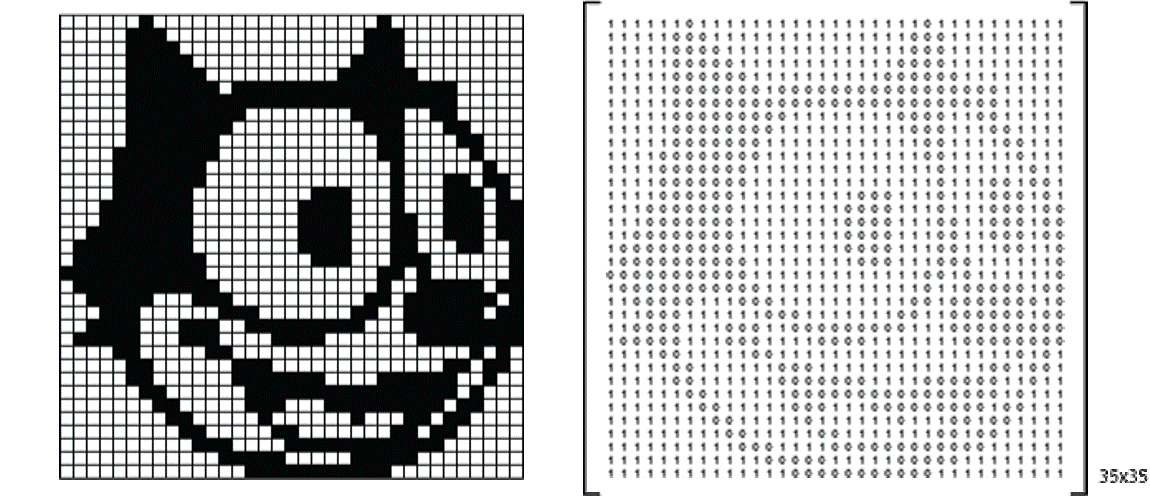
\includegraphics[width=9.5cm]{Figuras/Img01}
\end{center}


\end{frame}
%%%%%%%%%%%%%%%%%%%%%%%%%%%%%%%%%%%%%%%%%%%%%%%%%%%%%%%%

%%%%%%%%%%%%%%%%%%%%%%%%%%%%%%%%%%%%%%%%%%%%%%%%%%%%%%%%
\begin{frame}{El formato RGB}
    \begin{columns}
    \column{.5\textwidth}
    \begin{itemize}
        \item 
        Modelo de color basado en la síntesis aditiva
        \item 
        Es posible representar un color mediante la mezcla por adición de los tres colores de luz primarios: \textcolor{red}{rojo}, \textcolor{green}{verde} o \textcolor{azul}{azul}.
        \item 
        Tiene rangos de 0 a 255 (enteros) o de 0 a 1 (reales).
    \end{itemize}
    \column{.5\textwidth}
        \postitimg[6cm]{Figuras/Img02} % Inserta la figura correspondiente
    \end{columns}
\end{frame}
%%%%%%%%%%%%%%%%%%%%%%%%%%%%%%%%%%%%%%%%%%%%%%%%%%%%%%%%

%%%%%%%%%%%%%%%%%%%%%%%%%%%%%%%%%%%%%%%%%%%%%%%%%%%%%%%%
\begin{frame}{Ejemplo}
    \[
        R = \begin{pmatrix}
            0.0& 0.3& 0.9\\
            1.0& 0.0& 1.0
        \end{pmatrix};\quad
        G = \begin{pmatrix}
            0.0& 0.3& 0.3\\
            0.0& 1.0& 1.0
        \end{pmatrix};\quad
        B = \begin{pmatrix}
            0.0& 0.3& 0.9\\
            0.0& 0.0& 1.0
        \end{pmatrix}.
    \]
    \pause  
    \begin{center}
    \postitimg[5cm]{Figuras/Img03} % Inserta la figura correspondiente
    \end{center}
\end{frame}
%%%%%%%%%%%%%%%%%%%%%%%%%%%%%%%%%%%%%%%%%%%%%%%%%%%%%%%%

%%%%%%%%%%%%%%%%%%%%%%%%%%%%%%%%%%%%%%%%%%%%%%%%%%%%%%%%
\begin{frame}
    \frametitle{Reducción y Ampliación de Imágenes}

    \begin{columns}
    \column{.5\textwidth}
    \begin{block}{Reducción de Imágenes:}
        \begin{itemize}
            \item Proceso para disminuir el tamaño de una imagen.
            \item Puede provocar la pérdida de información al disminuir la cantidad de píxeles.
        \end{itemize}
    \end{block}
    
    \column{.5\textwidth}
    \begin{block}{Ampliación de Imágenes:}
        \begin{itemize}
            \item Proceso para aumentar el tamaño de una imagen.
            \item Generan píxeles adicionales que no estaban en la imagen original.
        \end{itemize}
    \end{block}
    
    \end{columns}

\end{frame}
%%%%%%%%%%%%%%%%%%%%%%%%%%%%%%%%%%%%%%%%%%%%%%%%%%%%%%%%


%%%%%%%%%%%%%%%%%%%%%%%%%%%%%%%%%%%%%%%%%%%%%%%%%%%%%%%%
\begin{frame}[fragile]
    \frametitle{Reducción de Imágenes}
    % \vspace{-1cm}
    \begin{center}
    % \begin{postitbox}[0.75\linewidth]
    \begin{tikzpicture}[->,>=stealth']
        % Right matrix J
        \matrix[matrix of nodes, nodes={draw, minimum size=1cm, anchor=center}, column sep=-\pgflinewidth, row sep=-\pgflinewidth] (J) {
            \node (5) {10}; & \node[fill=celeste!20] {13}; & \node (6) {20}; & \node {\dots}; \\
            \node[fill=celeste!20] {10}; & \node[fill=celeste!20] {25}; & \node[fill=celeste!20] {35}; & \node[fill=celeste!20] {\dots}; \\
            \node (7) {10}; & \node[fill=celeste!20] {25}; & \node (8) {40}; & \node {\dots}; \\
            \node {\dots}; & \node[fill=celeste!20] {\dots}; & \node {\dots}; & \node {\dots}; \\
        };

        
        % Left matrix I
        \matrix[matrix of nodes, nodes={draw, minimum size=1cm, anchor=center}, right=1.5cm of J, column sep=-\pgflinewidth, row sep=-\pgflinewidth] (I) {
            \node (1) {10}; & \node (2) {20}; & \node {\dots}; \\
            \node (3) {10}; & \node (4) {40}; & \node {\dots}; \\
            \node {\dots}; & \node {\dots}; & \node {\dots}; \\
        };
    
        % Curved arrow between the matrices with a slight upward bend
        % \draw[thick, color=azul!70] (1.north) to[out=10, in=110] (5.north);
        % \draw[thick, color=azul!70] (4.south) to[out=-10, in=-110] (8.south);
    
        % Arrow between I and J matrices
        \draw[thick] (J) -- (I);
    
    \end{tikzpicture}
    % \end{postitbox}
    \end{center}

\end{frame}


%%%%%%%%%%%%%%%%%%%%%%%%%%%%%%%%%%%%%%%%%%%%%%%%%%%%%%%%
\begin{frame}[fragile]
    \frametitle{Ampliación de Imágenes}
    \begin{center}
    % \begin{postitbox}[0.75\linewidth]
    \begin{tikzpicture}[->,>=stealth']
        % Left matrix I
        \matrix[matrix of nodes, nodes={draw, minimum size=1cm, anchor=center}, column sep=-\pgflinewidth, row sep=-\pgflinewidth] (I) {
            |[fill=celeste!20]| 10 & |[fill=celeste!20]| 20 & \dots \\
            |[fill=celeste!20]| 10 & |[fill=celeste!20]| 40 & \dots \\
            \dots & \dots & \dots \\
        };
    
        % Right matrix J
        \matrix[matrix of nodes, nodes={draw, minimum size=1cm, anchor=center}, right=1.5cm of I, column sep=-\pgflinewidth, row sep=-\pgflinewidth, nodes in empty cells] (J) {
            & & & & \\
            & |[fill=celeste!20]| 10 & \color{celeste} 15 & |[fill=celeste!20]| 20 & \dots \\
            & \color{celeste} 10 & \color{celeste} 20 & \color{celeste} 30 & \dots \\
            & |[fill=celeste!20]| 10 & \color{celeste} 25 & |[fill=celeste!20]| 40 & \dots \\
            & \dots & \dots & \dots & \dots \\
        };
    
        % Curved arrow between the matrices with a slight upward bend
        \draw[thick, color=azul!70] (I-1-1.north) to[out=10, in=135] (J-2-2);
        \draw[thick, color=azul!70] (I-2-2.south) to[out=-10, in=-135] (J-4-4);
    
        % Arrow between I and J matrices
        \draw[thick] (I) -- (J);
    
    \end{tikzpicture}
    % \end{postitbox}
    \end{center}

\end{frame}



%%%%%%%%%%%%%%%%%%%%%%%%%%%%%%%%%%%%%%%%%%%%%%%%%%%%%%%%
\begin{frame}

    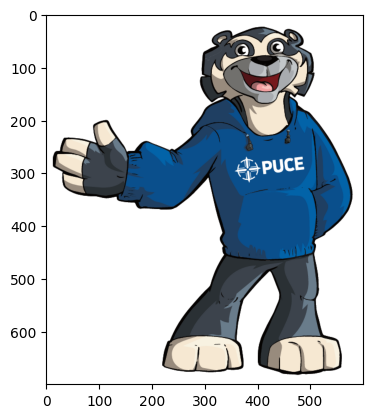
\includegraphics[width=5.4cm]{Figuras/output1.png}
    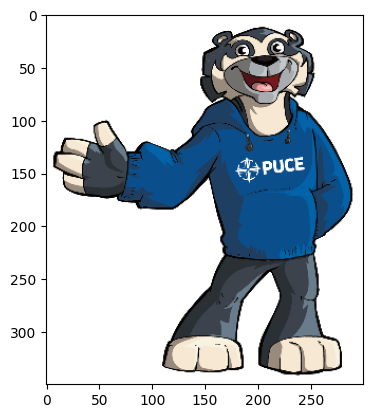
\includegraphics[width=2.7cm]{Figuras/output2.png}
    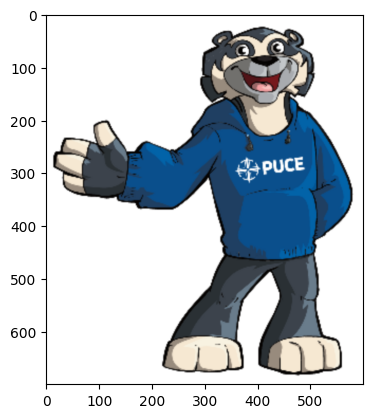
\includegraphics[width=5.4cm]{Figuras/output3.png}

\end{frame}

%%%%%%%%%%%%%%%%%%%%%%%%%%%%%%%%%%%%%%%%%%%%%%%%%%%%%%%%
\begin{frame}[fragile]
    \frametitle{Mejorar imágenes}

    \begin{center}
    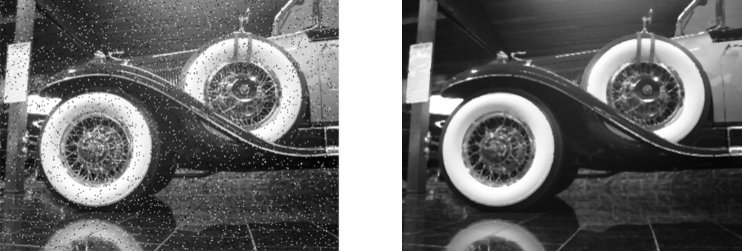
\includegraphics[width=9cm]{Figuras/Img04.png}

    \footnotesize
    \begin{tikzpicture}
    % Left matrix
    \matrix[matrix of nodes, nodes={draw, minimum size=0.8cm, anchor=center}, column sep=-\pgflinewidth, row sep=-\pgflinewidth] (A) {
        82 & 81 & 82\\
        81 & \color{purple}200 & 83 \\
        80 & 83 & 84 \\
    };
    
    % Green arrows pointing to the red value
    \foreach \i in {1,2,3} {
        \draw[->, thick, celeste, shorten >=-6pt, shorten <=-3pt] (A-\i-1) -- (A-2-2);
        \draw[->, thick, celeste, shorten >=-6pt, shorten <=-3pt] (A-\i-3) -- (A-2-2);
    }
    \foreach \i in {1,3} {
        \draw[->, thick, celeste, shorten >=-6pt, shorten <=-3pt] (A-\i-2) -- (A-2-2);
    }

    % Ordered list
    \node[draw, minimum height=0.8cm, right=4cm of A, anchor=center] (list) {
        \phantom{2}80 \quad 81 \quad 81 \quad 82 \quad \textcolor{celeste}{82} \quad 83 \quad 83 \quad 84 \quad 200
    };

    % Label 'Ordered List'
    \node[above=0.2cm of list] {Lista ordenada};

    % Arrow pointing to ordered list
    \draw[->, thick] (A) -- (list);

    % Arrow and label 'selected value'
    \draw[->, thick] (list.south) -- ++(0, -0.5) node[below] {valor seleccionado};

    % Right matrix
    \matrix[matrix of nodes, nodes={draw, minimum size=0.8cm, anchor=center}, right=8cm of A, column sep=-\pgflinewidth, row sep=-\pgflinewidth] (B) {
        \node {82}; & \node {81}; & \node {82}; \\
        \node {81}; & \node {\textcolor{celeste}{82}}; & \node {83}; \\
        \node {80}; & \node {83}; & \node {84}; \\
    };

    % Arrow pointing to right matrix
    \draw[->, thick] (list.east) -- (B);
\end{tikzpicture}

    \end{center}
\end{frame}

%%%%%%%%%%%%%%%%%%%%%%%%%%%%%%%%%%%%%%%%%%%%%%%%%%%%%%%%
\begin{frame}
    \frametitle{Un par más de conceptos}

    \begin{columns}
    \column{.5\textwidth}
    \begin{block}{Bounding Box}
        \begin{itemize}
            \item Delimita un objeto dentro de una imagen utilizando un rectángulo.
            \item Proporciona coordenadas $(x, y)$ y dimensiones $($ancho, alto$)$ del rectángulo.
        \end{itemize}
    \end{block}

    \column{.5\textwidth}

    \begin{tikzpicture}
    % Draw axes
    \draw[->, celeste] (-0.5,5) -- (4.5,5) node[right] {$x$};
    \draw[->, celeste] (0,5.5) -- (0,-0.5) node[right] {$y$};
    % (0,0) point and arrow
    \node[celeste, above left] at (0,5) {$(0,0)$};
    
    % Frame box
    \draw[thick, azul] (0,0) rectangle (4,5);
    
    % Bounding box
    \draw[thick, dashed] (1.5,3) rectangle (3,1);
    % (x,y) point and arrow
    \draw[dashed, celeste] (0,3) -- (1.5,3) -- (1.5,5);
    \fill[celeste] (1.5,3) circle (2pt);
    \node[celeste, above left] at (1.5,3) {$(x,y)$};
    
    \node at (2.25,2) {\scalebox{3.4}[5.2]{\color{azul}\faUmbrella}};
    \node[above right] at (1.5,3) {\footnotesize Bounding box};
    
    \draw[<->] (1.5,0.8) -- (3,0.8);
    \node[below] at (2.25,0.8) {\footnotesize ancho};
    
    \draw[<->] (3.2,1) -- (3.2,3);
    \node[right] at (3.2,2) {\rotatebox{90}{\footnotesize alto}};
    
    \end{tikzpicture}

    \end{columns}
    
\end{frame}
%%%%%%%%%%%%%%%%%%%%%%%%%%%%%%%%%%%%%%%%%%%%%%%%%%%%%%%%
%%%%%%%%%%%%%%%%%%%%%%%%%%%%%%%%%%%%%%%%%%%%%%%%%%%%%%%%
\begin{frame}
    \frametitle{Un par más de conceptos}

    \begin{columns}
    \column{.5\textwidth}
    \begin{block}{Segmentación Semántica}
        \begin{itemize}
            \item Asigna una etiqueta a cada píxel de la imagen, clasificándolos según el tipo de objeto al que pertenecen.
            \item Proporciona una delimitación precisa de los contornos de los objetos.
        \end{itemize}
    \end{block}
    \column{.5\textwidth}
    \begin{center}
        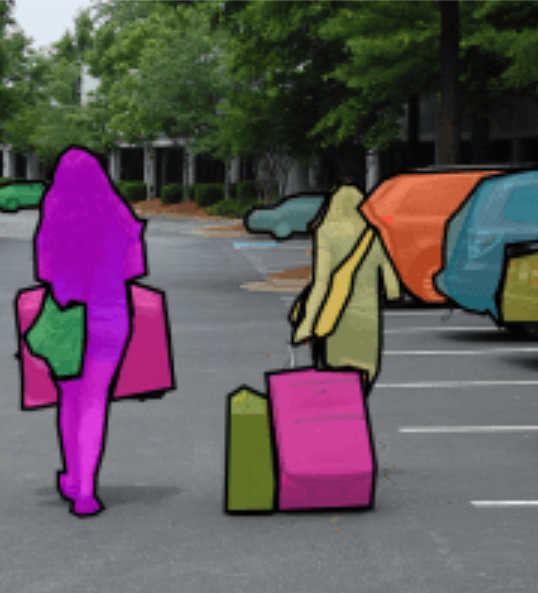
\includegraphics[width=5.5cm]{Figuras/Img05.png}
    \end{center}
    \end{columns}
    
\end{frame}
%%%%%%%%%%%%%%%%%%%%%%%%%%%%%%%%%%%%%%%%%%%%%%%%%%%%%%%%

% %%%%%%%%%%%%%%%%%%%%%%%%%%%%%%%%%%%%%%%%%%%%%%%%%%%%%%%%
\fondo{celeste}
\section{Convolución}
\fondo{blanco}
%%%%%%%%%%%%%%%%%%%%%%%%%%%%%%%%%%%%%%%%%%%%%%%%%%%%%%%%

%%%%%%%%%%%%%%%%%%%%%%%%%%%%%%%%%%%%%%%%%%%%%%%%%%%%%%%%
\begin{frame}
    \begin{block}{Convolución}
        La convolución entre dos funciones \( f \) y \( g \) se define como:
        \[
        s(t) = (f \ast g)(t) = \int_{-\infty}^{+\infty} f(\tau) g(t - \tau) \, d\tau
        \]
    \end{block}
    
    \begin{itemize}
        \item \( f \) es la función de entrada.
        \item \( g \) es el filtro o kernel.
    \end{itemize}
\end{frame}
%%%%%%%%%%%%%%%%%%%%%%%%%%%%%%%%%%%%%%%%%%%%%%%%%%%%%%%%


%%%%%%%%%%%%%%%%%%%%%%%%%%%%%%%%%%%%%%%%%%%%%%%%%%%%%%%%
\begin{frame}
    \begin{block}{Convolución Discreta}
        Para datos discretos, la convolución se define como:
        \[
        s(t) = (f \ast g)(t) = \sum_{\tau = -\infty}^{\infty} f(\tau) g(t - \tau)
        \]
    \end{block}
    
    \begin{block}{Convolución en Dos Dimensiones (Imágenes)}
        La convolución entre una imagen \( I \) y un kernel \( K \) es:
        \[
        S(i, j) = (I \ast K)(i, j) = \sum_m \sum_n I(i - m, j - n) K(m, n)
        \]
    \end{block}
\end{frame}
%%%%%%%%%%%%%%%%%%%%%%%%%%%%%%%%%%%%%%%%%%%%%%%%%%%%%%%%


%%%%%%%%%%%%%%%%%%%%%%%%%%%%%%%%%%%%%%%%%%%%%%%%%%%%%%%%
\begin{frame}
    \begin{block}{Correlación Cruzada}
        La correlación cruzada entre una imagen \( I \) y un kernel \( K \) es:
        \[
        S(i, j) = (I \ast K)(i, j) = \sum_m \sum_n I(i + m, j + n) K(m, n)
        \]
    \end{block}

    \begin{itemize}
        \item 
        En la práctica, se usa correlación cruzada en lugar de convolución.
        \item 
        La correlación cruzada evita invertir el kernel, lo que simplifica la implementación
    \end{itemize}
\end{frame}
%%%%%%%%%%%%%%%%%%%%%%%%%%%%%%%%%%%%%%%%%%%%%%%%%%%%%%%%



%%%%%%%%%%%%%%%%%%%%%%%%%%%%%%%%%%%%%%%%%%%%%%%%%%%%%%%%
\begin{frame}[fragile]
    \footnotesize
    \begin{tikzpicture}
        % Input matrix
        \matrix[matrix of math nodes, nodes={draw, minimum size=0.7cm, anchor=center, fill=celeste!20},column sep=-\pgflinewidth,row sep=-\pgflinewidth] (m1) {
            a & b & c & d \\
            e & f & g & h \\
            i & j & k & l \\
        };
    
        % Kernel matrix
        \matrix[matrix of math nodes, nodes={draw, minimum size=0.7cm, anchor=center, fill=gray!40},column sep=-\pgflinewidth,row sep=-\pgflinewidth] (m2) [right=0.5cm of m1] {
            w & x \\
            y & z \\
        };
    
        % Output matrix
        \matrix[matrix of math nodes,nodes={draw, minimum size=0.7cm, minimum width=3cm, anchor=center},column sep=-\pgflinewidth,row sep=-\pgflinewidth] (m3) [right=0.5cm of m2] {
            aw+bx+ey+fz & bw+cx+fy+gz & cw+dx+gy+hz \\
            ew+fx+iy+jz & fw+gx+jw+kz & gw+hx+ky+lz \\
        };
    
        % Labels
        \node[below=0.2cm of m1] {Input ($3\times4$)};
        \node[below=0.2cm of m2] {Kernel ($2\times2$)};
        \node[below=0.2cm of m3] {Output ($2\times3$)};
    
        % Dashed boxes around convolution areas
        \draw[red, thick, dashed] ($(m1-1-1.north west)+(-0.1,0.1)$)  rectangle ($(m1-2-2.south east)+(0.1,-0.1)$);
        \draw[red, thick, dashed] ($(m2-1-1.north west)+(-0.1,0.1)$)  rectangle ($(m2-2-2.south east)+(0.1,-0.1)$);
        \draw[red, thick, dashed] ($(m3-1-1.north west)+(-0.1,0.1)$) rectangle ($(m3-1-1.south east)+(0.1,-0.1)$);
    
        % Arrows
        \draw[red, thick, ->] ($(m1-1-1.north east)+(0,0.1)$) to[out=10, in=150] ($(m3-1-1.north)+(0.4,0.1)$);
        \draw[red, thick, ->] ($(m2-1-1.north east)+(0,0.1)$) to[out=10, in=140] ($(m3-1-1.north)+(-0.4,0.1)$);
    
        % Operations
        \node[right=-0.05cm of m1] {\large $*$};
        \node[right=-0.05cm of m2] {\large $=$};
        
    \end{tikzpicture}
\end{frame}

\begin{frame}{Filtros}

    \vspace*{-2.5cm}
    \begin{columns}
    \column{3cm}
        
        \href{https://mlnotebook.github.io/img/CNN/convSobel.gif}{Ver animación.}
        
    \column{8cm}
    \begin{center}
        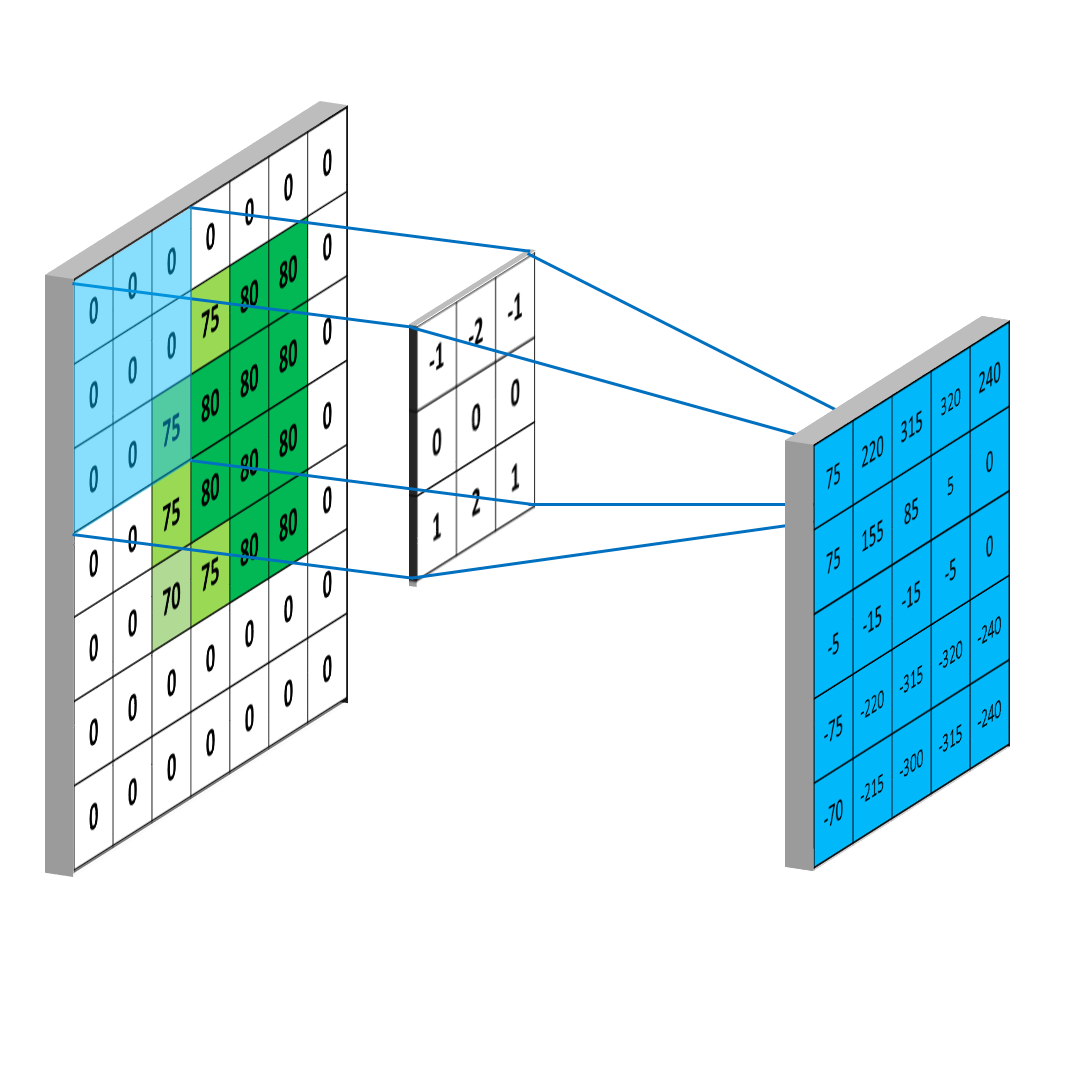
\includegraphics[height=9.5cm]{Figuras/Fig10}
    \end{center}
    \end{columns}
    
\end{frame}

%%%%%%%%%%%%%%%%%%%%%%%%%%%%%%%%%%%%%%%%%%%%%%%%%%%%%%%%
\begin{frame}

    La dimensión de salida después de aplicar una convolución es:
    \[
        (I_1 - K_1 + 1,\ I_2 - K_2 + 1),
    \]
    dónde
    \begin{itemize}
        \item 
        \( I_1, I_2 \) son las dimensiones de la imagen de entrada, y 
        \item 
        \( K_1, K_2 \) son las dimensiones del kernel
    \end{itemize}
\end{frame}
%%%%%%%%%%%%%%%%%%%%%%%%%%%%%%%%%%%%%%%%%%%%%%%%%%%%%%%%

% %%%%%%%%%%%%%%%%%%%%%%%%%%%%%%%%%%%%%%%%%%%%%%%%%%%%%%%%
\fondo{celeste}
\section{Redes convolucionales}
\fondo{blanco}
%%%%%%%%%%%%%%%%%%%%%%%%%%%%%%%%%%%%%%%%%%%%%%%%%%%%%%%%


%%%%%%%%%%%%%%%%%%%%%%%%%%%%%%%%%%%%%%%%%%%%%%%%%%%%%%%%
\begin{frame}
    \frametitle{Redes convolucionales}

    \begin{itemize}
        \item Se inspiran en la corteza visual de los animales.
        \item Desarrollo desde Neocognitron (Fukushima, 1982) a LeNet-5 (LeCun, 1989).
        \item Avance impulsado por hardware mejorado y algoritmos optimizados a partir de 2012.
        \item CNNs aplican filtros convolucionales para extraer patrones como bordes, texturas, y formas a diferentes niveles de abstracción.
    \end{itemize}

    
\end{frame}
%%%%%%%%%%%%%%%%%%%%%%%%%%%%%%%%%%%%%%%%%%%%%%%%%%%%%%%%

%%%%%%%%%%%%%%%%%%%%%%%%%%%%%%%%%%%%%%%%%%%%%%%%%%%%%%%%
\begin{frame}
\centering
    \postitimg[12cm]{Figuras/FigDL.png}
\end{frame}
%%%%%%%%%%%%%%%%%%%%%%%%%%%%%%%%%%%%%%%%%%%%%%%%%%%%%%%%

%%%%%%%%%%%%%%%%%%%%%%%%%%%%%%%%%%%%%%%%%%%%%%%%%%%%%%%%
\begin{frame}
    \frametitle{Capa de Convolución}

    \begin{itemize}[leftmargin=*]
    \item Se hace mediante la aplicación de Filtros.
    \item El filtro es la matriz de pesos de una capa de convolución dentro de una CNN.
    \item  Si se tiene 3 canales, se aplica un filtro por canar y se suman los resultados de la siguiente manera:
    \[
        R*K_1 + G*K_2 + B*K_3.
    \]
    \item El kernel siempre tiene el mismo número de canales que la entrada.
    \end{itemize}
    
\end{frame}
%%%%%%%%%%%%%%%%%%%%%%%%%%%%%%%%%%%%%%%%%%%%%%%%%%%%%%%%

%%%%%%%%%%%%%%%%%%%%%%%%%%%%%%%%%%%%%%%%%%%%%%%%%%%%%%%%
\begin{frame}
\centering
    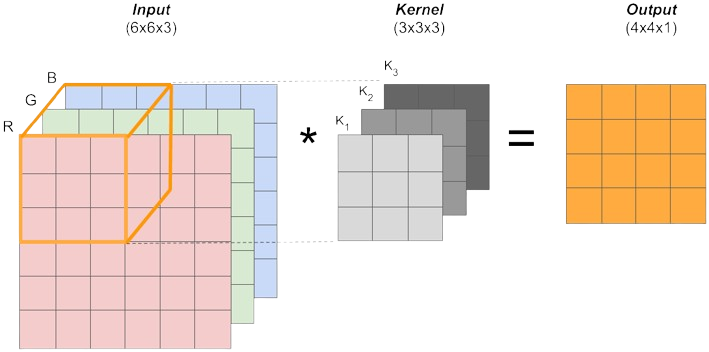
\includegraphics[width=0.9\linewidth]{Figuras/Img06.png}
\end{frame}
%%%%%%%%%%%%%%%%%%%%%%%%%%%%%%%%%%%%%%%%%%%%%%%%%%%%%%%%

%%%%%%%%%%%%%%%%%%%%%%%%%%%%%%%%%%%%%%%%%%%%%%%%%%%%%%%%
\begin{frame}
\centering
    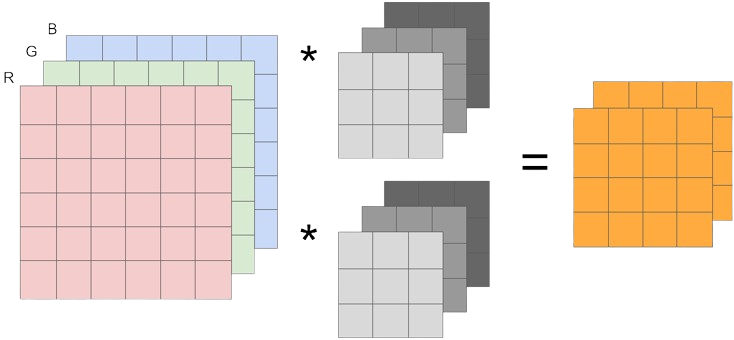
\includegraphics[width=0.9\linewidth]{Figuras/Img07.png}
\end{frame}
%%%%%%%%%%%%%%%%%%%%%%%%%%%%%%%%%%%%%%%%%%%%%%%%%%%%%%%%

%%%%%%%%%%%%%%%%%%%%%%%%%%%%%%%%%%%%%%%%%%%%%%%%%%%%%%%%
\begin{frame}
    \frametitle{Dimensiones}

    \begin{itemize}
        \item Entrada: $(n_w,n_h,n_c)$.
        \item Kernel: $(n_{k_1},n_{k_2},n_c)$.
        \item Número de kernels: $n$.
        \item Salida: 
        \[
            (n_w - n_{k_1} + 1,\ n_h - n_{k_2} + 1,\ n).
        \]
    \end{itemize}
    
\end{frame}
%%%%%%%%%%%%%%%%%%%%%%%%%%%%%%%%%%%%%%%%%%%%%%%%%%%%%%%%


%%%%%%%%%%%%%%%%%%%%%%%%%%%%%%%%%%%%%%%%%%%%%%%%%%%%%%%%
\begin{frame}
    \frametitle{Padding (Relleno)}

    Evita la reducción del tamaño de la salida agregando ceros alrededor de la entrada.

    \centering
    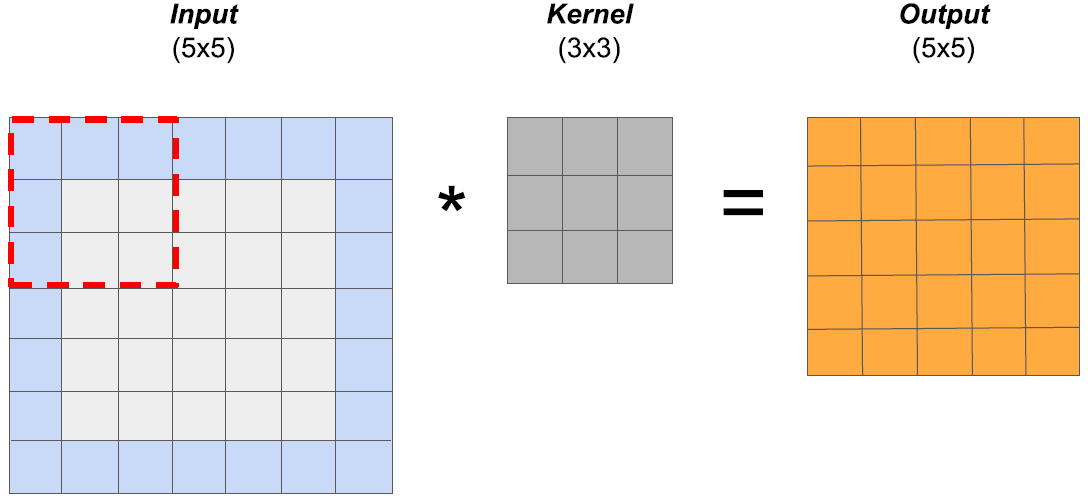
\includegraphics[width=0.67\linewidth]{Figuras/Img08.png}
\end{frame}
%%%%%%%%%%%%%%%%%%%%%%%%%%%%%%%%%%%%%%%%%%%%%%%%%%%%%%%%

%%%%%%%%%%%%%%%%%%%%%%%%%%%%%%%%%%%%%%%%%%%%%%%%%%%%%%%%
\begin{frame}
    \frametitle{Dimensiones}

    \begin{itemize}
        \item Entrada: $(n_w,n_h)$.
        \item Kernel: $(n_k,n_k)$.
        \item Valor de relleno: $p$.
        \item Salida: 
        \[
            (n_w-n_k+2p+1,\ n_h-n_k+2p+1)
        \]
    \end{itemize}

    Para mantener el tamaño de la entrada, el padding \(p\) se calcula como:
    \[
        p = \left\lfloor \frac{n_k - 1}{2} \right\rfloor
    \]
    
\end{frame}
%%%%%%%%%%%%%%%%%%%%%%%%%%%%%%%%%%%%%%%%%%%%%%%%%%%%%%%%

%%%%%%%%%%%%%%%%%%%%%%%%%%%%%%%%%%%%%%%%%%%%%%%%%%%%%%%%
\begin{frame}
    \frametitle{Convoluciones por Pasos (Stride)}

    Aplican la operación de convolución saltando celdas en la entrada.
    
    \centering
    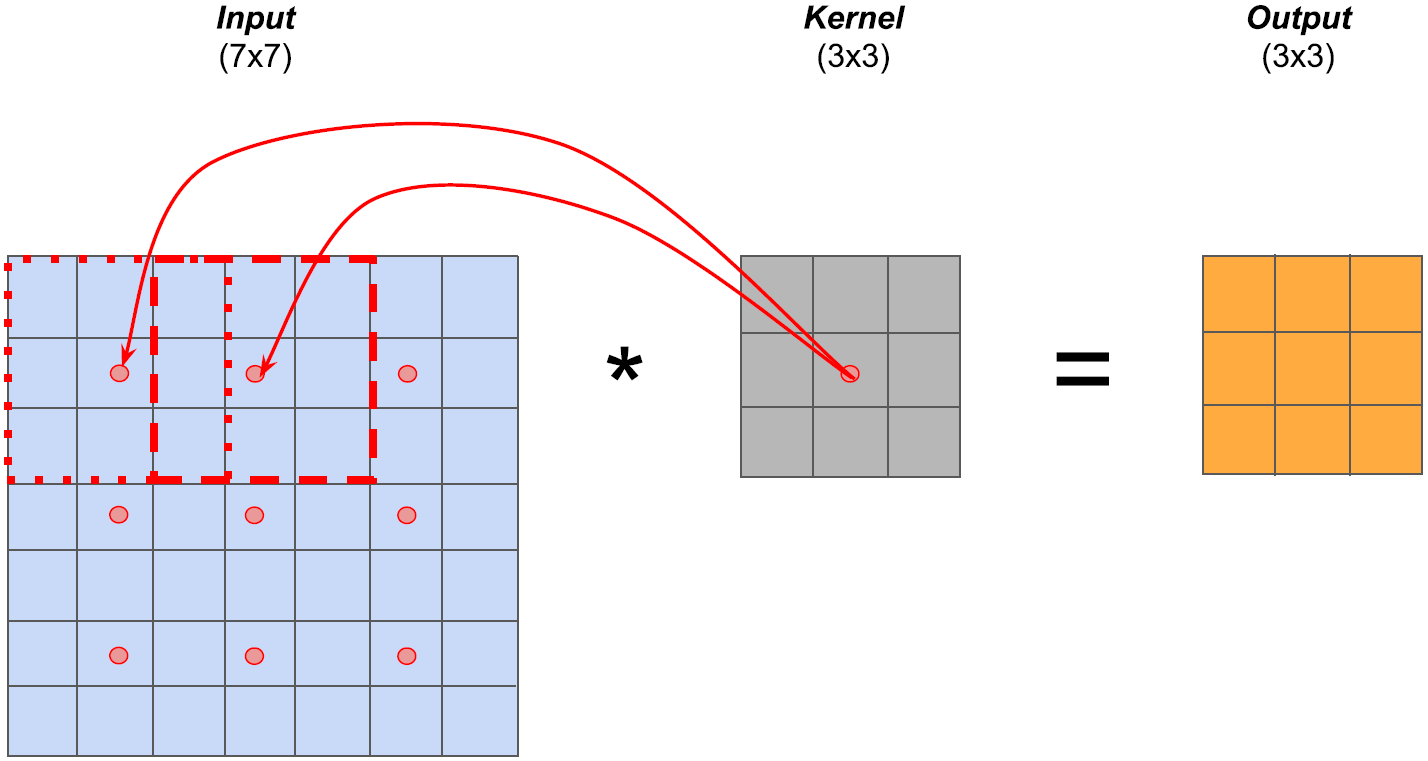
\includegraphics[width=0.67\linewidth]{Figuras/Img09.png}

\end{frame}
%%%%%%%%%%%%%%%%%%%%%%%%%%%%%%%%%%%%%%%%%%%%%%%%%%%%%%%%

%%%%%%%%%%%%%%%%%%%%%%%%%%%%%%%%%%%%%%%%%%%%%%%%%%%%%%%%
\begin{frame}
    \frametitle{Dimensiones}

    \begin{itemize}
        \item Entrada: $(n_w,n_h)$.
        \item Kernel: $(n_k,n_k)$.
        \item Valor de relleno: $p$.
        \item Paso o stride: $s$
        \item Salida: 
        \[
            \left(\left\lfloor \frac{n_w - n_k + 2p}{s} + 1 \right\rfloor ,\  \left\lfloor \frac{n_h - n_k + 2p}{s} + 1 \right\rfloor\right)
        \]
    \end{itemize}

    Reduce la dimensión de la salida al aplicar un mayor paso en la convolución.

\end{frame}
%%%%%%%%%%%%%%%%%%%%%%%%%%%%%%%%%%%%%%%%%%%%%%%%%%%%%%%%

%%%%%%%%%%%%%%%%%%%%%%%%%%%%%%%%%%%%%%%%%%%%%%%%%%%%%%%%
\begin{frame}[fragile]
    \frametitle{Capa de Agrupamiento (Pooling)}
    Reducen la dimensión de los datos de entrada.

    \begin{columns}
    \column{.5\textwidth}
    \begin{block}{Max-pooling}Valor máximo en una región de la entrada.\phantom{g}
    \end{block}
    \column{.5\textwidth}
    \begin{block}{Average-pooling}Promedio de los valores en una región.
    \end{block}
    \end{columns}

    \begin{center}
        \small
    \begin{tikzpicture}
    % Input matrix
    \matrix[matrix of math nodes,nodes={draw, minimum size=0.6cm, anchor=center, fill=celeste!40},column sep=-\pgflinewidth,row sep=-\pgflinewidth] (m1) {
        1 & 3 & 2 & 1 \\
        2 & 9 & 1 & 1 \\
        1 & 3 & 2 & 3 \\
        5 & 6 & 1 & 2 \\
    };

    % Output matrix
    \matrix[matrix of math nodes,nodes={draw, minimum size=0.6cm, anchor=center, fill=celeste!40},column sep=-\pgflinewidth,row sep=-\pgflinewidth] (m2) [right=1cm of m1] {
        9 & 2 \\
        6 & 3 \\
    };


    % Dashed boxes for pooling regions (Input)
    \draw[azul, thick, dashed] ($(m1-1-1.north west)+(-0.01,0.01)$)  rectangle ($(m1-2-2.south east)+(0.01,-0.01)$);
    \draw[purple, thick, dashed] ($(m1-1-3.north west)+(-0.01,0.01)$)  rectangle ($(m1-2-4.south east)+(0.01,-0.01)$);
    \draw[brown, thick, dashed] ($(m1-3-1.north west)+(-0.01,0.01)$)  rectangle ($(m1-4-2.south east)+(0.01,-0.01)$);
    \draw[teal, thick, dashed] ($(m1-3-3.north west)+(-0.01,0.01)$)  rectangle ($(m1-4-4.south east)+(0.01,-0.01)$);

    % Dashed boxes for pooling regions (Output)
    \draw[azul, thick, dashed] ($(m2-1-1.north west)+(-0.01,0.01)$) rectangle ($(m2-1-1.south east)+(0.01,-0.01)$);
    \draw[purple, thick, dashed] ($(m2-1-2.north west)+(-0.01,0.01)$) rectangle ($(m2-1-2.south east)+(0.01,-0.01)$);
    \draw[brown, thick, dashed] ($(m2-2-1.north west)+(-0.01,0.01)$) rectangle ($(m2-2-1.south east)+(0.01,-0.01)$);
    \draw[teal, thick, dashed] ($(m2-2-2.north west)+(-0.01,0.01)$) rectangle ($(m2-2-2.south east)+(0.01,-0.01)$);

    % Arrow from Input to Output
    \draw[->, thick] ($(m1.east)$) -- ($(m2.west)$);

    \draw[azul, thick, ->] ($(m1-1-1.north east)+(0,0.1)$) to[out=20, in=150] ($(m2-1-1.north)+(0,0.1)$);
    \end{tikzpicture}
    \end{center}
\end{frame}
%%%%%%%%%%%%%%%%%%%%%%%%%%%%%%%%%%%%%%%%%%%%%%%%%%%%%%%%

%%%%%%%%%%%%%%%%%%%%%%%%%%%%%%%%%%%%%%%%%%%%%%%%%%%%%%%%
\begin{frame}
    \frametitle{Estructura de una Red Neuronal Convolucional (CNN)}

    \begin{itemize}[leftmargin=*]
        \item \textbf{Bloque convolucional:}
        \begin{itemize}[leftmargin=*]
            \item Incluye capas de convolución, agrupamiento (pooling) y activación.
            \item Detecta patrones y características en los datos de entrada.
        \end{itemize}

        \item \textbf{Bloque totalmente conectado:}
        \begin{itemize}[leftmargin=*]
            \item Cada neurona se conecta con todas las neuronas de la capa anterior y siguiente.
            \item Correlacionan las características detectadas por las capas convolucionales.
        \end{itemize}

        \item \textbf{Bloque de decisión:}
        \begin{itemize}[leftmargin=*]
            \item Genera un vector de probabilidades para cada clase.
            \item Usa funciones como softmax.
        \end{itemize}
    \end{itemize}

\end{frame}
%%%%%%%%%%%%%%%%%%%%%%%%%%%%%%%%%%%%%%%%%%%%%%%%%%%%%%%%


%%%%%%%%%%%%%%%%%%%%%%%%%%%%%%%%%%%%%%%%%%%%%%%%%%%%%%%%
\begin{frame}[fragile]
    \frametitle{Estructura de una Red Neuronal Convolucional (CNN)}

    \begin{center}
\tikzstyle{block} = [rectangle, draw, rounded corners, minimum width=1cm, minimum height=3cm, node distance=2cm]
\begin{tikzpicture}
    % Blocks
    \node (data) {Datos};
    \node (conv) [block, right of=data, fill=green!20] {\rotatebox{90}{Bloque Convolucional}};
    \node (fc) [block, right of=conv, fill=gray!20] {\rotatebox{90}{Bloque totalmente conectado}};
    \node (softmax) [block, right of=fc, fill=red!20] {\rotatebox{90}{Bloque de decisión}};
    \node[right=of softmax] (results) {Resultados};

    % Arrows
    \draw[->] (data) -- (conv);
    \draw[->] (conv) -- (fc);
    \draw[->] (fc) -- (softmax);
    \draw[->] (softmax) -- (results);

\end{tikzpicture}
    \end{center}
\end{frame}
%%%%%%%%%%%%%%%%%%%%%%%%%%%%%%%%%%%%%%%%%%%%%%%%%%%%%%%%


%%%%%%%%%%%%%%%%%%%%%%%%%%%%%%%%%%%%%%%%%%%%%%%%%%%%%%%%
\begin{frame}[fragile]
    \frametitle{Estructura de una Red Neuronal Convolucional (CNN)}

    \begin{center}\small
\begin{tikzpicture}
    % Data block (Input)
    \node[minimum height=2.9cm, label=above:Input, minimum width=1.4cm] (data) {\rotatebox{90}{\textbf{Datos}}};
    
    % Convolutional block
    \node[draw=teal, fill=teal!10, right=0.5cm of data, minimum width=6cm, minimum height=3cm, label={[text=teal]above:Convolucional}] (convblock) {};
    
    % FC block
    \node[draw=gray, fill=gray!10, right=1cm of convblock, minimum width=1.5cm, minimum height=3cm, label={[text=gray]above:T. Conectada}] (fc) {};
    
    % Softmax block
    \node[draw=purple, fill=purple!10, right=1cm of fc, minimum width=1cm, minimum height=3cm, label={[text=purple]above:Decisión}] (softmax) {};
    
    % Convolutional layers inside convolutional block
    \node[draw=teal, minimum width=0.7cm, minimum height=2cm] (conv) at ($(convblock.west)+(0.8,0)$) {\rotatebox{90}{\color{teal}Convolución}};
    \node[draw=teal, minimum width=0.7cm, minimum height=2cm, right=0.3cm of conv] (pool) {\rotatebox{90}{\color{teal}Relleno}};
    \node[draw=teal, minimum width=0.7cm, minimum height=2cm, right=0.3cm of pool] (act) {\rotatebox{90}{\color{teal}Activación}};

    % Capa 1
    \draw[dashed, color=teal] ($(conv.west)+(-0.2,-1.3)$) rectangle ($(act.east)+(0.2,1.3)$);
    \node[below=0.5cm of pool] {\color{teal}Capa 1};
    
    % Puntos
    \node[right=0.5cm of act] (dots) {$\cdots$};

    % Capa n
    \draw[dashed, color=teal] ($(act.east)+(1.5,-1.3)$) rectangle ($(act.east)+(2.5,1.3)$);
    \node at ($(act.east)+(2,-1.8)$) {\color{teal}Capa $n$};

    % Arrow connections Convolucional
    \draw[->, thick] (data.east) -- (convblock.west);
    \draw[->, thick, teal] ($(act.east)+(0.2,0)$) -- (dots.west);
    \draw[<-, thick, teal] ($(act.east)+(1.5,0)$) -- (dots.east);

    
    % FC connections
    \node (a1) at ($(convblock.east)+(0,1)$) [inner sep=0pt]{};
    \node (a2) at ($(convblock.east)$) [inner sep=0pt]{};
    \node (a3) at ($(convblock.east)+(0,-1)$) [inner sep=0pt]{};

    \foreach \i in {-1.25,-1,...,1.25} {
        \foreach \a in {a1, a2, a3} {
            \draw[line width=0.2pt, color=gray] (\a) -- ($(fc.west)+(0.4,+\i)$);
        }
        \foreach \j in {-0.75,-0.25,...,0.75} {
            \draw[line width=0.2pt, color=gray] ($(fc.west)+(0.4,+\i)$) -- ($(fc.west)+(1.1,+\j)$);
        }
        \node at ($(fc.west)+(0.4,+\i)$) [circle, fill=gray, inner sep=1.2pt]{};
    }
    
    \foreach \j in {1,0,-1} {
        \node at ($(softmax.west)+(0.5,+\j)$) [circle, fill=purple, inner sep=1.2pt]{};
        \foreach \i in {-0.75,-0.25,...,0.75} {
            \draw[line width=0.2pt, color=purple] ($(fc.west)+(1.1,+\i)$) -- ($(softmax.west)+(0.5,+\j)$);
            \node at ($(fc.west)+(1.1,+\i)$) [circle, fill=gray, inner sep=1.2pt]{};
        }
        \draw[->, thick] ($(softmax.east)+(0,\j)$) -- ++(0.5,0);
    
    }

    % Data block (Input)
    \node[minimum height=2.9cm, minimum width=1.4cm, label=above:Output, right=0.5cm of softmax] {\rotatebox{90}{\textbf{Resultado}}};
\end{tikzpicture}
    \end{center}
\end{frame}
%%%%%%%%%%%%%%%%%%%%%%%%%%%%%%%%%%%%%%%%%%%%%%%%%%%%%%%%


%%%%%%%%%%%%%%%%%%%%%%%%%%%%%%%%%%%%%%%%%%%%%%%%%%%%%%%%
\begin{frame}
    \frametitle{Ejemplo de una CNN: LeNet-5}
    
    \centering
    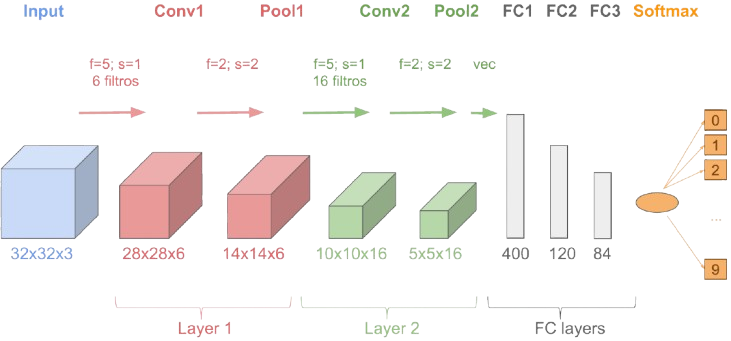
\includegraphics[width=0.9\linewidth]{Figuras/Img11.png}

\end{frame}
%%%%%%%%%%%%%%%%%%%%%%%%%%%%%%%%%%%%%%%%%%%%%%%%%%%%%%%%

%%%%%%%%%%%%%%%%%%%%%%%%%%%%%%%%%%%%%%%%%%%%%%%%%%%%%%%%
\begin{frame}
    \frametitle{Capa de Entrada (Input Layer)}
    
    \begin{itemize}
        \item La capa de entrada recibe la imagen (o los datos de entrada) y la prepara para su procesamiento.
        \item No hay parámetros que aprender en esta capa.
        \item La imagen se representa como una matriz de píxeles, que puede ser en escala de grises o RGB.
    \end{itemize}

\end{frame}
%%%%%%%%%%%%%%%%%%%%%%%%%%%%%%%%%%%%%%%%%%%%%%%%%%%%%%%%

%%%%%%%%%%%%%%%%%%%%%%%%%%%%%%%%%%%%%%%%%%%%%%%%%%%%%%%%
\begin{frame}
    \frametitle{Capas Convolucionales (Convolutional Layers)}

    \begin{itemize}
        \item Una capa convolucional tiene \( l \) canales de entrada, \( k \) canales de salida, y un tamaño de filtro \( f \).
        \item El número total de pesos es:
        \[
        f \times f \times l \times k
        \]
        \item Además, cada mapa de características tiene un valor de sesgo, por lo tanto, el número total de parámetros es:
        \[
        f \times f \times (l + 1) \times k
        \]
    \end{itemize}
    
\end{frame}
%%%%%%%%%%%%%%%%%%%%%%%%%%%%%%%%%%%%%%%%%%%%%%%%%%%%%%%%

%%%%%%%%%%%%%%%%%%%%%%%%%%%%%%%%%%%%%%%%%%%%%%%%%%%%%%%%
\begin{frame}
    \frametitle{Capas de Agrupamiento (Pooling Layers)}

    \begin{itemize}
        \item Las capas de agrupamiento (pooling) se encargan de reducir las dimensiones de las características, haciéndolas más manejables.
        \item No hay parámetros que aprender durante el proceso de entrenamiento en estas capas.
    \end{itemize}

\end{frame}
%%%%%%%%%%%%%%%%%%%%%%%%%%%%%%%%%%%%%%%%%%%%%%%%%%%%%%%%

%%%%%%%%%%%%%%%%%%%%%%%%%%%%%%%%%%%%%%%%%%%%%%%%%%%%%%%%
\begin{frame}
    \frametitle{Capas Totalmente Conectadas (Fully-Connected Layers)}

    \begin{itemize}
        \item En las capas totalmente conectadas, cada unidad de entrada se conecta con todas las unidades de salida.
        \item El número de pesos es \( n \times m \), donde \( n \) es el número de entradas y \( m \) el número de salidas.
        \item Además, cada neurona de salida tiene un valor de sesgo, por lo tanto, el número total de parámetros es:
        \[
        (n + 1) \times m
        \]
    \end{itemize}

\end{frame}
%%%%%%%%%%%%%%%%%%%%%%%%%%%%%%%%%%%%%%%%%%%%%%%%%%%%%%%%

%%%%%%%%%%%%%%%%%%%%%%%%%%%%%%%%%%%%%%%%%%%%%%%%%%%%%%%%
\begin{frame}
    \frametitle{Capa de Salida (Output Layer)}

    \begin{itemize}
        \item La capa de salida es generalmente una capa totalmente conectada.
        \item Genera las probabilidades o clasificaciones finales.
        \item El número total de parámetros en la capa de salida también es:
        \[
        (n + 1) \times m
        \]
    \end{itemize}

\end{frame}
%%%%%%%%%%%%%%%%%%%%%%%%%%%%%%%%%%%%%%%%%%%%%%%%%%%%%%%%

%%%%%%%%%%%%%%%%%%%%%%%%%%%%%%%%%%%%%%%%%%%%%%%%%%%%%%%%
\begin{frame}
    \centering
    \begin{tabular}{ccrr}
    \toprule
    \textbf{Capa}  & \textbf{Dimensión} & \textbf{Tamaño} & \textbf{Parámetros} \\ 
    \midrule
    Input   & $(32 \times 32 \times 3)$   & 3072   & 0        \\
    Conv1   & $(28 \times 28 \times 6)$   & 4704   & 456      \\ 
    Pool1   & $(14 \times 14 \times 6)$   & 1176   &         \\ 
    Conv2   & $(10 \times 10 \times 16)$  & 1600   &     \\ 
    Pool2   & $(5 \times 5 \times 16)$    & 400     &         \\ 
    FC2     & $(120 \times 1)$       & 120     &    \\ 
    FC3     & $(84 \times 1)$        & 84      &    \\ 
    Softmax & $(10 \times 1)$        & 10      &       \\ 
    \midrule
    Total &&&\\
    \bottomrule
    \end{tabular}

\end{frame}
%%%%%%%%%%%%%%%%%%%%%%%%%%%%%%%%%%%%%%%%%%%%%%%%%%%%%%%%

%%%%%%%%%%%%%%%%%%%%%%%%%%%%%%%%%%%%%%%%%%%%%%%%%%%%%%%%
\begin{frame}
    \centering
    \begin{tabular}{ccrr}
    \toprule
    \textbf{Capa}  & \textbf{Dimensión} & \textbf{Tamaño} & \textbf{Parámetros} \\ 
    \midrule
    Input   & $(32 \times 32 \times 3)$   & 3072   & 0        \\
    Conv1   & $(28 \times 28 \times 6)$   & 4704   & 456      \\ 
    Pool1   & $(14 \times 14 \times 6)$   & 1176   & 0        \\ 
    Conv2   & $(10 \times 10 \times 16)$  & 1600   & 2416    \\ 
    Pool2   & $(5 \times 5 \times 16)$    & 400     & 0        \\ 
    FC2     & $(120 \times 1)$       & 120     & 48120   \\ 
    FC3     & $(84 \times 1)$        & 84      & 10164   \\ 
    Softmax & $(10 \times 1)$        & 10      & 850      \\ 
    \midrule
    Total &&&62006\\
    \bottomrule
    \end{tabular}

\end{frame}
%%%%%%%%%%%%%%%%%%%%%%%%%%%%%%%%%%%%%%%%%%%%%%%%%%%%%%%%

% %%%%%%%%%%%%%%%%%%%%%%%%%%%%%%%%%%%%%%%%%%%%%%%%%%%%%%%%
\fondo{celeste}
\section{Arquitecturas de CNN}
\fondo{blanco}
%%%%%%%%%%%%%%%%%%%%%%%%%%%%%%%%%%%%%%%%%%%%%%%%%%%%%%%%

%%%%%%%%%%%%%%%%%%%%%%%%%%%%%%%%%%%%%%%%%%%%%%%%%%%%%%%%
\begin{frame}
    \frametitle{LeNet-5}

    \begin{columns}
    
    \column{.4\textwidth}
    \begin{center}
        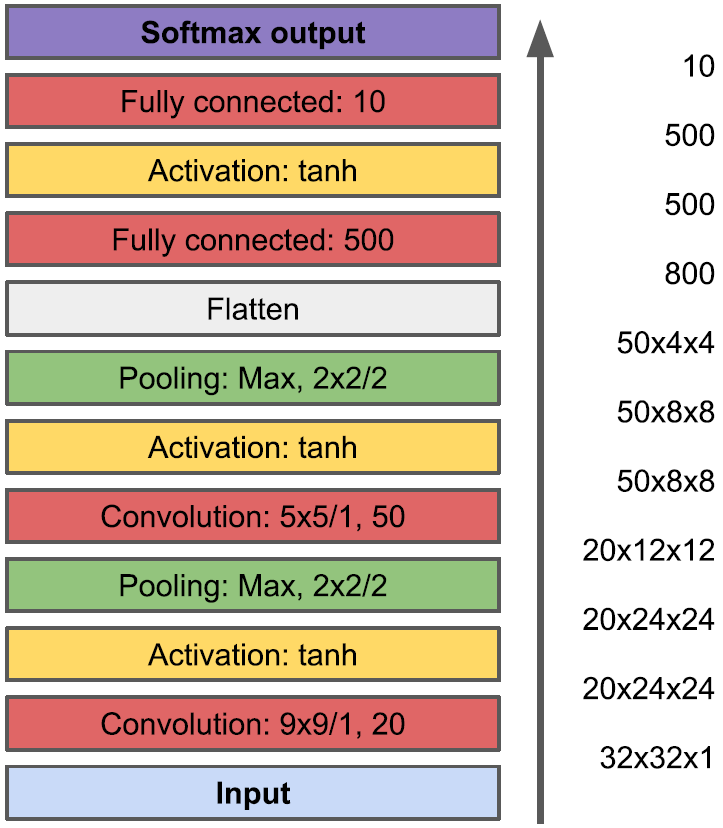
\includegraphics[width=0.9\linewidth]{Figuras/Img12.png}
    \end{center}
    
    \column{.6\textwidth}
    \begin{itemize}
        \item Desarrollada por Bengio et al. en 1998.
        \item Objetivo: reconocimiento de dígitos escritos a mano.
        \item Pequeña y eficiente.
        \item Ideal para aprender y realizar pruebas iniciales.
        \item Puede ejecutarse en una CPU sin necesidad de GPU.
    \end{itemize}

    \end{columns}

\end{frame}
%%%%%%%%%%%%%%%%%%%%%%%%%%%%%%%%%%%%%%%%%%%%%%%%%%%%%%%%


%%%%%%%%%%%%%%%%%%%%%%%%%%%%%%%%%%%%%%%%%%%%%%%%%%%%%%%%
\begin{frame}
\frametitle{AlexNet}
\centering
    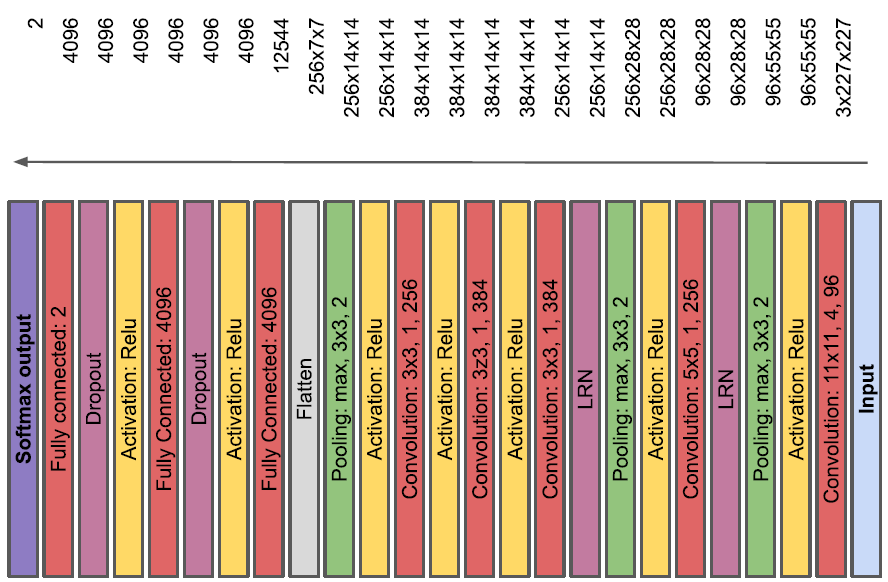
\includegraphics[width=0.65\linewidth]{Figuras/Img13.png}
\end{frame}
%%%%%%%%%%%%%%%%%%%%%%%%%%%%%%%%%%%%%%%%%%%%%%%%%%%%%%%%

%%%%%%%%%%%%%%%%%%%%%%%%%%%%%%%%%%%%%%%%%%%%%%%%%%%%%%%%
\begin{frame}
\frametitle{VGG}
\centering
    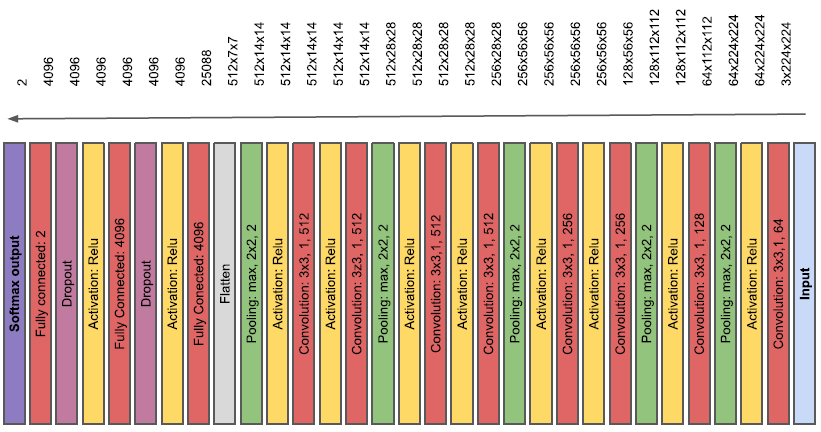
\includegraphics[width=0.8\linewidth]{Figuras/Img14.png}
\end{frame}
%%%%%%%%%%%%%%%%%%%%%%%%%%%%%%%%%%%%%%%%%%%%%%%%%%%%%%%%

%%%%%%%%%%%%%%%%%%%%%%%%%%%%%%%%%%%%%%%%%%%%%%%%%%%%%%%%
\begin{frame}
\frametitle{YOLOv5}
\centering
    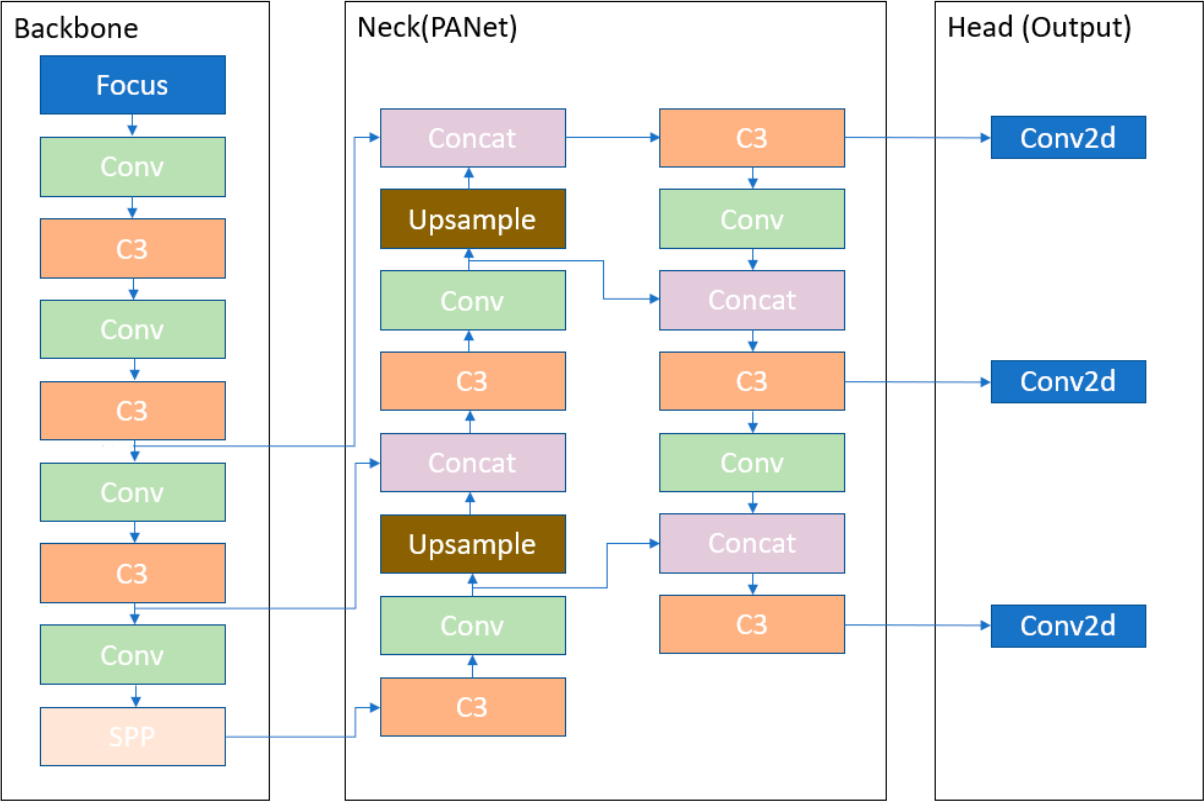
\includegraphics[width=0.65\linewidth]{Figuras/yolov5.png}
\end{frame}
%%%%%%%%%%%%%%%%%%%%%%%%%%%%%%%%%%%%%%%%%%%%%%%%%%%%%%%%


%%%%%%%%%%%%%%%%%%%%%%%%%%%%%%%%%%%%%%%%%%%%%%%%%%%%%%%%
\begin{frame}
    \frametitle{Transferencia del Aprendizaje}

    \begin{itemize}[leftmargin=*]
        \item Permite reutilizar un modelo entrenado en una tarea para aplicarlo en otra tarea similar.
        \item Mejora el rendimiento del modelo y acelera el progreso.
        \item Es popular en **Deep Learning** debido a los altos costos computacionales y de datos necesarios para entrenar modelos desde cero.
        \item La técnica más común es usar un \textbf{modelo pre-entrenado} y adaptarlo:
        \begin{itemize}
            \item Seleccionar el modelo fuente.
            \item Reutilizar todo o parte del modelo.
            \item Ajustar el modelo a la nueva tarea (tunning).
        \end{itemize}
    \end{itemize}

\end{frame}
%%%%%%%%%%%%%%%%%%%%%%%%%%%%%%%%%%%%%%%%%%%%%%%%%%%%%%%%

%%%%%%%%%%%%%%%%%%%%%%%%%%%%%%%%%%%%%%%%%%%%%%%%%%%%%%%%
\begin{frame}
    \frametitle{Técnicas de ajuste (tunning)}

        \begin{itemize}
            \item \textbf{Extracción de características:} usar el modelo como extractor de características.
            \item \textbf{Congelación de capas:} mantener los pesos de algunas capas y reentrenar otras.
        \end{itemize}


\end{frame}
%%%%%%%%%%%%%%%%%%%%%%%%%%%%%%%%%%%%%%%%%%%%%%%%%%%%%%%%


%%%%%%%%%%%%%%%%%%%%%%%%%%%%%%%%%%%%%%%%
%% Página final
\fondo{final}
\begin{frame}[plain]
\begin{center}
    \color{white}
    
    \vspace{1.5cm}
    {\Huge\textbf{Gracias}}
    \vspace{2mm}
    
\tikzset{
  qrcode/.style = {line width = 2sp},
  pixel on/.style = {azul},
  pixel off/.style = {azul},
}

    \begin{tabular}{ccc}\color{azul}
        \qrcode[hyperlink,height=2.5cm,version=5]{https://linktr.ee/aemerinot}
        &\phantom{.\hspace{.5cm}.}&
        \qrcode[hyperlink,height=2.5cm,version=5]{https://github.com/andres-merino/Presentacion-ChatGPT-AulaInvertida}
        \\ \\
        \LARGE \faLinkedin\hspace{5mm} \faGithub%\hspace{5mm} \aiOrcidSquare 
        && 
        Presentación
    \end{tabular}

    \vspace{2mm}
    \textbf{Contacto:} aemerinot@puce.edu.ec
\end{center}
\end{frame}


\end{document}